\documentclass[]{article}
\usepackage{lmodern}
\usepackage{amssymb,amsmath}
\usepackage{ifxetex,ifluatex}
\usepackage{fixltx2e} % provides \textsubscript
\ifnum 0\ifxetex 1\fi\ifluatex 1\fi=0 % if pdftex
  \usepackage[T1]{fontenc}
  \usepackage[utf8]{inputenc}
\else % if luatex or xelatex
  \ifxetex
    \usepackage{mathspec}
  \else
    \usepackage{fontspec}
  \fi
  \defaultfontfeatures{Ligatures=TeX,Scale=MatchLowercase}
\fi
% use upquote if available, for straight quotes in verbatim environments
\IfFileExists{upquote.sty}{\usepackage{upquote}}{}
% use microtype if available
\IfFileExists{microtype.sty}{%
\usepackage{microtype}
\UseMicrotypeSet[protrusion]{basicmath} % disable protrusion for tt fonts
}{}
\usepackage[margin=1in]{geometry}
\usepackage{hyperref}
\hypersetup{unicode=true,
            pdftitle={Is there a relation between women attractivness and their perceived intelligence?},
            pdfborder={0 0 0},
            breaklinks=true}
\urlstyle{same}  % don't use monospace font for urls
\usepackage{graphicx,grffile}
\makeatletter
\def\maxwidth{\ifdim\Gin@nat@width>\linewidth\linewidth\else\Gin@nat@width\fi}
\def\maxheight{\ifdim\Gin@nat@height>\textheight\textheight\else\Gin@nat@height\fi}
\makeatother
% Scale images if necessary, so that they will not overflow the page
% margins by default, and it is still possible to overwrite the defaults
% using explicit options in \includegraphics[width, height, ...]{}
\setkeys{Gin}{width=\maxwidth,height=\maxheight,keepaspectratio}
\IfFileExists{parskip.sty}{%
\usepackage{parskip}
}{% else
\setlength{\parindent}{0pt}
\setlength{\parskip}{6pt plus 2pt minus 1pt}
}
\setlength{\emergencystretch}{3em}  % prevent overfull lines
\providecommand{\tightlist}{%
  \setlength{\itemsep}{0pt}\setlength{\parskip}{0pt}}
\setcounter{secnumdepth}{0}
% Redefines (sub)paragraphs to behave more like sections
\ifx\paragraph\undefined\else
\let\oldparagraph\paragraph
\renewcommand{\paragraph}[1]{\oldparagraph{#1}\mbox{}}
\fi
\ifx\subparagraph\undefined\else
\let\oldsubparagraph\subparagraph
\renewcommand{\subparagraph}[1]{\oldsubparagraph{#1}\mbox{}}
\fi

%%% Use protect on footnotes to avoid problems with footnotes in titles
\let\rmarkdownfootnote\footnote%
\def\footnote{\protect\rmarkdownfootnote}

%%% Change title format to be more compact
\usepackage{titling}

% Create subtitle command for use in maketitle
\newcommand{\subtitle}[1]{
  \posttitle{
    \begin{center}\large#1\end{center}
    }
}

\setlength{\droptitle}{-2em}
  \title{Is there a relation between women attractivness and their perceived
intelligence?}
  \pretitle{\vspace{\droptitle}\centering\huge}
  \posttitle{\par}
  \author{}
  \preauthor{}\postauthor{}
  \date{}
  \predate{}\postdate{}


\begin{document}
\maketitle

{
\setcounter{tocdepth}{2}
\tableofcontents
}
\subsection{Hypothesis}\label{hypothesis}

There is an opinion that the more attractive women, the less they are
burdened by their intelligence. Author's private experince didn't find a
confirmation of such a thesis, however, it appeared to be interesting to
refute it using a larger sample. The goal of this reasearch is to verify
a hypothesis that attracive women are actually percevied to be more
intelligent by men than their less attractive fellows.

\subsection{Dataset overview}\label{dataset-overview}

To verify a hypothesis an appropriate dataset was chosen. The dataset
\footnote{\url{http://www.stat.columbia.edu/~gelman/arm/examples/speed.dating/}}
was gathered by Columbia Business School from multiple speed dating
\footnote{\url{https://en.wikipedia.org/wiki/Speed_dating}} events from
2002-2004 in USA and consists from 8378 rows. Each row in the dataset
represents a short 4 minute date. A date has 195 various attributes, but
only a few will be of our interest: \emph{gender} to distinguish women,
\emph{attr\_o}- attractiveness rated by the partner and \emph{intel\_o}-
intelligence rated by the partner. To allow easier analysis let's
extract from the dataset only rows containing women attributes rated by
men and select only two columns we're interested in: \emph{attr\_o} and
\emph{intel\_o}. For the sake of readability let's rename them to
\emph{attractiveness} and \emph{intelligence} respectively. Finally,
let's remove rows which have NA values. As a result, we have a dataset
with 4029 rows and 2 columns: \emph{attractiveness} and
\emph{intelligence}.

\subsection{Dataset visualisation}\label{dataset-visualisation}

Let's first visualise our dataset and see if we can find any insights.
Since our variables are discrete, a standard scatter plot may be
misleading because points would be overlapping. To prevent overplotting
we'll apply jittering \footnote{\url{http://ggplot2.tidyverse.org/reference/geom_jitter.html}}
to the points. \emph{Figure 1} shows a relation between female
attractivness and intelligence. Apparently, there is no strong linear
correlation between attractivness and inteligence (correlation
coefficient is 0.42 with p-value close to
1.3319033\times 10\^{}\{-170\}). However, we can observe that there is a
pattern- the further we go by \emph{attractivness} axis, the less low
scores for \emph{intelligence} we can see. And vice versa- the lower
score for \emph{attractivness}, the less high scores for
\emph{intelligence}. Let's find out if this observation is statistically
significant.
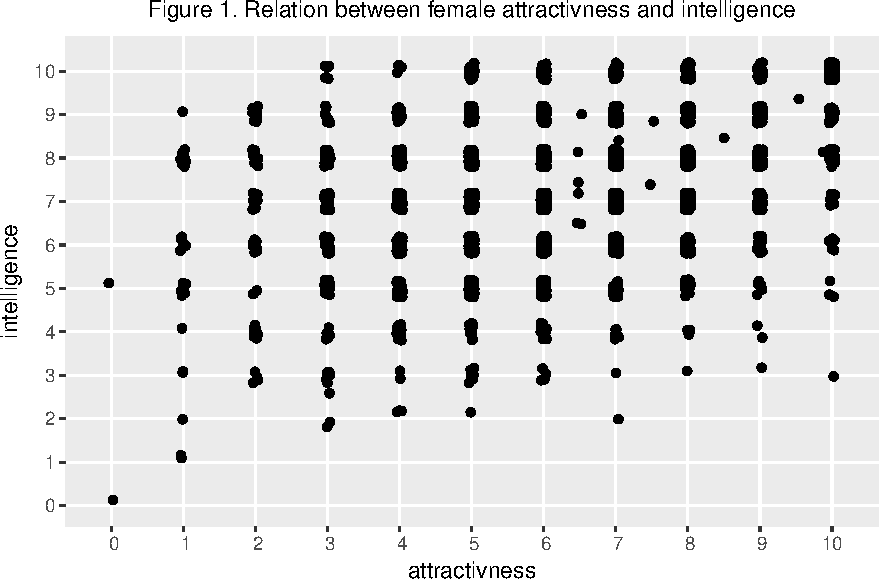
\includegraphics{FemaleAttractivenessAndIntelligence_files/figure-latex/unnamed-chunk-4-1.pdf}

\subsection{Hypothesis testing}\label{hypothesis-testing}

To test our hypothesis let's select two, approximately equally sized,
groups from our dataset. The first group will be consisting of women
whoes appearence was rated from 0 to 5, and the second group with
appereance from 8 to 10. Distribution characteristics of both groups are
depicted in \emph{Figure 2}.

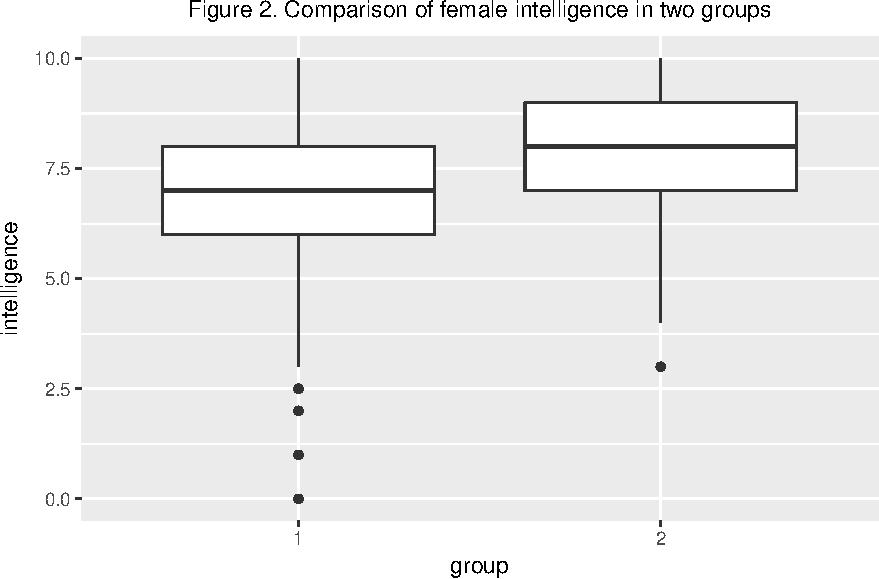
\includegraphics{FemaleAttractivenessAndIntelligence_files/figure-latex/unnamed-chunk-6-1.pdf}

Now it is time to formalise our hypothesis.

\emph{Null hypothesis}- there is no difference in mean perceived
intelligince between two groups of women- less and more attractive.

\emph{Alternative hypothesis}- mean perceived intelligence in the group
with more attractive women is greater than in the group with less
attractive women.

Let's perform a two-sample one-tailed Student's t-test with 95\%
confidence level. Mean intelligence in the first group appears to be
6.59, in the second group- 8.07. p-value is
\(2.4089975\times 10^{-120}\) which is much less than 0.05 (for 95\%
confidence level) thus allowing us to reject the null hypothesis in
favour of the alternative hypothesis.

\subsection{Conclusion}\label{conclusion}

Even though there is no strong linear correlation between women
attractivness and their intelligence, on average, more attractive women
are perceived by men to be more intelligent.


\end{document}
